
\documentclass{beamer}
\usecolortheme{dove}
\setbeamertemplate{navigation symbols}{}
\usepackage{amsmath,amssymb,amsfonts,amsthm, multicol, subfigure, color}
\usepackage{bm}
\usepackage{graphicx}
\usepackage{tabularx}
\usepackage{booktabs}
\usepackage{hyperref}
\usepackage{pdfpages}
\usepackage{xcolor}
\definecolor{seagreen}{RGB}{46, 139, 87}
\def\independenT#1#2{\mathrel{\rlap{$#1#2$}\mkern2mu{#1#2}}}
\newcommand\indep{\protect\mathpalette{\protect\independenT}{\perp}}
\def\log{\text{log}}
\newcommand\logit{\text{logit}}
\newcommand\iid{\stackrel{\text{iid}}{\sim}}
\newcommand\E{\text{E}}
\newcommand\V{\text{V}}
\renewcommand\P{\text{P}}
\newcommand{\Cov}{\text{Cov}}
\newcommand{\Cor}{\text{Cor}}
\newcommand\doop{\texttt{do}}
\usepackage{stackrel}
\usepackage{tikz}
\usetikzlibrary{arrows,shapes.arrows,positioning,shapes,patterns,calc}
\newcommand\slideref[1]{\vskip .1cm \tiny \textcolor{gray}{{#1}}}
\newcommand\red[1]{\color{red}#1}
\newcommand\blue[1]{\color{blue}#1}
\newcommand\gray[1]{\color{gray}#1}
\newcommand\seagreen[1]{\color{seagreen}#1}
\newcommand\purple[1]{\color{purple}#1}
\newcommand\orange[1]{\color{orange}#1}
\newcommand\black[1]{\color{black}#1}
\newcommand\white[1]{\color{white}#1}
\newcommand\teal[1]{\color{teal}#1}
\newcommand\magenta[1]{\color{magenta}#1}
\newcommand\Fuchsia[1]{\color{Fuchsia}#1}
\newcommand\BlueGreen[1]{\color{BlueGreen}#1}
\newcommand\bblue[1]{\textcolor{blue}{\textbf{#1}}}
\newcommand\bred[1]{\textcolor{red}{\textbf{#1}}}
\newcommand\bgray[1]{\textcolor{gray}{\textbf{#1}}}
\newcommand\bgreen[1]{\textcolor{seagreen}{\textbf{#1}}}
\newcommand\bref[2]{\href{#1}{\color{blue}{#2}}}
\colorlet{lightgray}{gray!40}
\pgfdeclarelayer{bg}    % declare background layer for tikz
\pgfsetlayers{bg,main} % order layers for tikz
\newcommand\mycite[1]{\begin{scriptsize}\textcolor{darkgray}{(#1)}\end{scriptsize}}
\newcommand{\tcframe}{
\begin{frame}{Causal Inference in Observational Settings}
\scriptsize{
\only<1|handout:0>{\tableofcontents}
\only<2|handout:1>{\tableofcontents[currentsection]}
}
\end{frame}
}

\newcommand{\tcsubframe}{
\begin{frame}{Causal Inference in Observational Settings}
\scriptsize{
\tableofcontents[currentsubsection]
}
\end{frame}
}

\usepackage[round]{natbib}
\bibliographystyle{humannat-mod}
\setbeamertemplate{enumerate items}[default]
\usepackage{mathtools}
\usepackage{ulem}
\usepackage{cancel}


\newcommand{\goalsframe}{\begin{frame}{Learning goals for the semester}
At the end of the semester, you will be able to:
\begin{itemize}
    \item evaluate the credibility of causal claims
    \item answer causal questions in your own research
    \item engage with new methods for causal inference
\end{itemize} \vskip .2in
\end{frame}}

\title{27--28. Semester Review}
\author{Ian Lundberg\\Cornell Info 6751: Causal Inference in Observational Settings\\Fall 2022}
\date{29 Nov and 1 Dec 2022}

\begin{document}

\maketitle

\goalsframe


\section{Causal claims require an argument}

\tcframe

\begin{frame}{Causal claims require an argument}

\includegraphics[width = .6\textwidth]{figures/Biles_bar}
\includegraphics[width = .3\textwidth]{figures/Biles_medal}

\vskip .2in
\begin{tiny}
Left photo: By Fernando Frazão/Agência Brasil - \url{http://agenciabrasil.ebc.com.br/sites/_agenciabrasil2013/files/fotos/1035034-_mg_0802_04.08.16.jpg, CC BY 3.0 br, https://commons.wikimedia.org/w/index.php?curid=50548410} \\
Right photo: By Agencia Brasil Fotografias - EUA levam ouro na ginástica artística feminina; Brasil fica em 8 lugar, CC BY 2.0, \url{https://commons.wikimedia.org/w/index.php?curid=50584648}\\
\end{tiny}

\end{frame}

\begin{frame}{Causal claims require an argument}
\begin{enumerate}
\item Statistical evidence
\begin{itemize}
\item Simone Biles swung on the uneven bars. She won a gold medal. \pause
\item I did not swing on the uneven bars. I did not win a gold medal.
\end{itemize} \pause
\item Possible causal claim
\begin{itemize}
\item Swinging on the uneven bars causes a person to win a gold medal.
\end{itemize}
\end{enumerate} \vskip .2in \pause
\begin{tabular}{rccc}
& \multicolumn{2}{l}{Do you win gold if you:} & Causal effect \\
& Swing & Do not swing & of swinging \\
\hline
Simone Biles & Yes (1) & \only<1-4>{?}\only<5->{\blue{No (0)}} & \only<1-5>{?}\only<6->{+1} \\
Ian & \only<1-6>{?}\only<7->{\blue{No (0)}} & No (0) & \only<1-7>{?}\only<8->{0} \\
\hline
\end{tabular}
\end{frame}

\section{Causal inference without models (nonparametric)}

\tcframe

\subsection{Consistency}

\begin{frame}{Consistency} \pause
\begin{tikzpicture}[x = \textwidth, y = .8\textheight]
\draw[thick] (0,.6) -- (.4, .6) -- (.4,0);
\node[anchor = south] at (.2,0) {Potential Outcomes};
\node at (.1,.4) {$Y_i^1$};
\node at (.2,.4) {$Y_i^2$};
\node at (.15,.3) {$Y_i^3$};
\node at (.25,.3) {$Y_i^4$};
\onslide<3->{\draw[thick] (1,.6) -- (.6, .6) -- (.6,0);
\node[anchor = south] at (.8,0) {Factual Outcomes};
\node at (.8,.35) {$Y_i$};
}
\onslide<4->{
\node[anchor = south, align = center, blue, draw, rounded corners, line width = 1.2pt, inner sep = 12pt] at (.5,.65) {Consistency Assumption\\$Y_i^{A_i} = Y_i$};
}
\end{tikzpicture}
\end{frame}

\begin{frame}{Consistency}
$$Y_i = Y_i^{A_i}$$
The factual outcome $Y_i$ equals the potential outcome $Y_i^{A_i}$ under the factual treatment $A_i$ \vskip .2in
Requires
\begin{enumerate}
\item Potential outcomes are well-defined
\item Treatments are measured in observed data
\end{enumerate}
\end{frame}

\begin{frame}{Consistency Threat: Interference} \pause

\begin{center}\includegraphics[width = .5\textwidth]{figures/nike_vaporfly}\\\begin{tiny}Image source: \href{https://www.nike.com/t/zoomx-vaporfly-next-2-mens-road-racing-shoes-glWqfm}{Nike}\end{tiny}\end{center} \pause

Suppose my challenger is a tiny bit faster than me \pause
\begin{center}
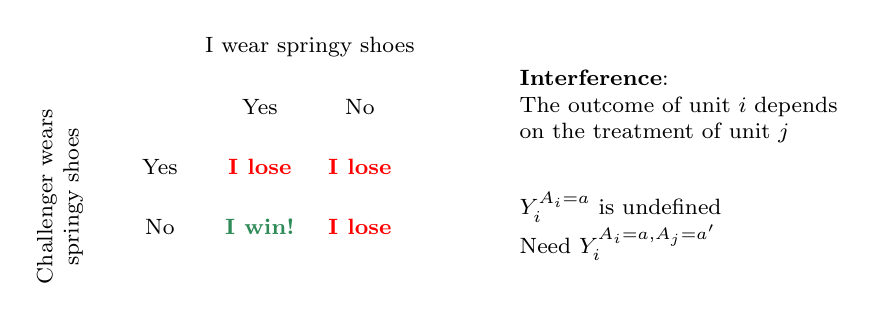
\begin{tikzpicture}[x = .5in, y = .3in]
\node[rotate = 90, align = center, font = {\footnotesize}] at (-1,-1.5) {Challenger wears\\springy shoes};
\node[font = \footnotesize] at (0,-1) {Yes};
\node[font = \footnotesize] at (0,-2) {No};
\node[font = {\footnotesize}] at (1.5,1) {I wear springy shoes};
\node[font = \footnotesize] at (1,0) {Yes};
\node[font = \footnotesize] at (2,0) {No}; \pause
\node[font = {\footnotesize\bf}, red] at (1,-1) {I lose};
\node[font = {\footnotesize\bf}, red] at (2,-1) {I lose}; \pause
\node[font = {\footnotesize\bf}, seagreen] at (1,-2) {I win!};
\node[font = {\footnotesize\bf}, red] at (2,-2) {I lose}; \pause
\node[align = left, anchor = west, font = \footnotesize] at (3.5,0) {\textbf{Interference}:\\The outcome of unit $i$ depends\\on the treatment of unit $j$}; \pause
\node[align = left, anchor = west, font = \footnotesize] at (3.5,-2) {$Y_i^{A_i=a}$ is undefined\\Need $Y_i^{A_i=a,A_j=a'}$};
\end{tikzpicture}
\end{center}
\end{frame}

\begin{frame}{Consistency Threat: Variations of Treatment} \pause

\begin{itemize}
\item Finding: A Cornell degree causes higher earnings,\\compared to no college degree \pause
\item For-profit college makes an ad:
\begin{itemize}
\item Pay us lots of money
\item Evidence shows a degree will raise your earnings
\end{itemize}
\end{itemize} \pause \vskip .1in
\bgray{Problem}: The college you attend is relevant \vskip .1in \pause

Formally, you can collapse treatments only if we believe\\treatment variation irrelevance \bref{https://doi.org/10.1097/EDE.0b013e3181bd5638}{(VanderWeele 2009)}
$$Y_i^{a,k_a} = Y_i^{a,k'_a}\quad\text{for all}\quad k_a,k'_a$$
where
\begin{itemize}
\item $a$ is the treatment \hfill college degree
\item $k_a$ and $k'_a$ are versions \hfill which college
\end{itemize}
\end{frame}

\begin{frame}{Consistency. Summary}

$$Y_i^{A_i} = Y_i$$ \vskip .2in \pause

Consistency holds when
\begin{itemize}
\item potential outcomes are well-defined and
\item treatment is measured
\end{itemize} \vskip .2in \pause
Consistency would not hold to the degree that
\begin{itemize}
\item The outcome of unit $i$ depends on the treatment of unit $j$
\item The treatment $A_i$ is a coarse aggregation over relevant version
\end{itemize} \vskip .2in \pause
Those settings require careful definitions of the potential outcomes \vskip .2in \pause
\bred{Important:} Consistency is a concern that \bblue{precedes} confounding
\begin{itemize}
\item First define the treatment and outcome
\item Then move on to subsequent assumptions
\end{itemize}

\end{frame}

\subsection{Exchangeability}

\begin{frame}{Exchangeability} \pause
\begin{center}
\includegraphics[width = \textwidth]{figures/diamonds} \\ \pause
\end{center}
\bblue{Exchangeability.} Under randomization, the left equals the right:
$$\E(Y^{a=1} - Y^{a=0}) = \E(Y\mid A = 1) - \E(Y\mid A = 0)$$
\end{frame}

\begin{frame}{Exchangeability: In math}
Exchangeability: $A\indep \{Y^a\}$
\begin{itemize}
\item Treatment is independent of potential outcomes
\item Achieved in expectation in a simple randomized experiment
\end{itemize} \vskip .2in

Conditional exchangeability: $A\indep \{Y^a\}\mid \vec{L}$
\begin{itemize}
\item Treatment is independent of potential outcomes\\within strata of $\vec{L}$
\item Achieved in expectation in a randomized experiment with unequal assignment probabilities that are a function of $\vec{L}$
\end{itemize}

\end{frame}

\begin{frame}{Exchangeability: Using DAGs}

$A$ and $Y$ are associated through two paths
\begin{itemize}
\onslide<2->{\item A \bblue{causal path} $A\rightarrow Y$}
\onslide<3->{\item A \bred{backdoor path} $A \leftarrow C\rightarrow Y$}
\begin{itemize}
\onslide<4->{\item Think of a house at $A$}
\onslide<5->{\item Walk out the back door to $C$, then around the house to $Y$}
\end{itemize}
\end{itemize}
\begin{center}
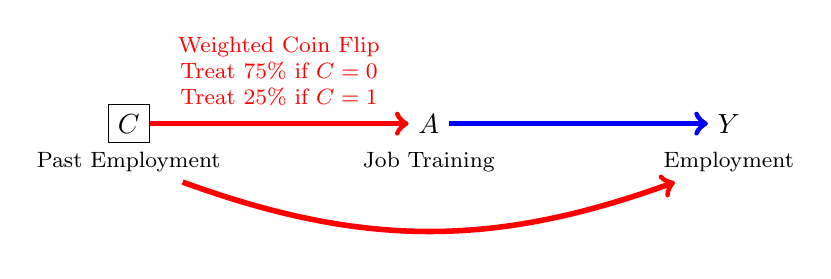
\begin{tikzpicture}[x = 1.5in, y = .5in]
\onslide<1->{
\node (a) at (0,0) {$A$};
\node (y) at (1,0) {$Y$};
\node[anchor = north, font = \footnotesize] (alab) at (a.south) (0,0) {Job Training};
\node[anchor = north, font = \footnotesize] (ylab) at (y.south) {Employment};
\draw[->, line width = 2pt, blue] (a) -- (y);
}
\onslide<1->{
\node[align = center] (c) at (-1,0) {$C$};
\node[font = \footnotesize, align = center, anchor = north] (clab) at (c.south) {Past Employment};
\draw[->, line width = 2pt, red] (c) -- node[midway, above, align = center, font = \footnotesize, outer sep = 3pt] {Weighted Coin Flip\\Treat 75\% if $C = 0$\\Treat 25\% if $C = 1$} (a);
\draw[->, line width = 2pt, red] (clab) to[bend right = 20] (ylab);
}
\draw<6-> (c.south west) rectangle (c.north east);
\end{tikzpicture}
\end{center}
\onslide<6->{To block the backdoor path, condition on $C$}
\begin{itemize}
\onslide<6->{\item Analyze within strata of $C$}
\onslide<6->{\item Denoted by the box}
\end{itemize}
\end{frame}

\begin{frame}{Exchangeability: Using DAGs}

Three sources of association in DAGs
\begin{enumerate}
\item Causal path: $A\rightarrow Y$, $A\rightarrow M\rightarrow Y$, etc.
\item Backdoor path: $A\leftarrow L\rightarrow Y$
\begin{itemize}
\item Conditioning on $L$ blocks the path
\end{itemize}
\item Path through an adjusted collider: $A\rightarrow \boxed{C}\leftarrow Y$
\begin{itemize}
\item Conditioning on $C$ opens the path
\end{itemize}
\end{enumerate} \vskip .2in

The effect $A\rightarrow Y$ is identified if the only source of association between $A$ and $Y$ comes from causal paths

\end{frame}

\begin{frame}{Exchangeability: Using DAGs}

What adjustment set identifies the total effect of $A$ on $Y$?
\begin{itemize}
\item (3 correct answers)
\end{itemize}
\begin{center}
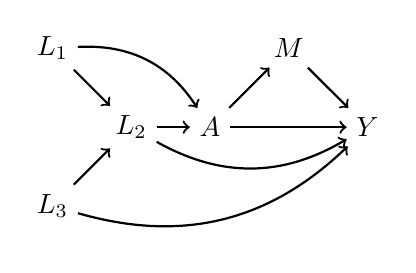
\begin{tikzpicture}
\node (a) at (0,0) {$A$};
\node (m) at (1,1) {$M$};
\node (y) at (2,0) {$Y$};
\node (l1) at (-2,1) {$L_1$};
\node (l2) at (-1,0) {$L_2$};
\node (l3) at (-2,-1) {$L_3$};
\draw[->, thick] (a) -- (m);
\draw[->, thick] (m) -- (y);
\draw[->, thick] (a) -- (y);
\draw[->, thick] (l1) -- (l2);
\draw[->, thick] (l1) to[bend left] (a);
\draw[->, thick] (l2) -- (a);
\draw[->, thick] (l2) to[bend right] (y);
\draw[->, thick] (l3) -- (l2);
\draw[->, thick] (l3) to[bend right] (y);
\end{tikzpicture}
\end{center} \pause
\begin{itemize}
\item We have to condition on $L_2$ to block $A\leftarrow L_2\rightarrow Y$ \pause
\item That opens the path $A\leftarrow L_1\rightarrow \boxed{L_2}\leftarrow L_3\rightarrow Y$ \pause
\item We can block that by conditioning on $L_1$, $L_3$, or both \pause
\end{itemize} \vskip .05in
Three sufficient sets: $\{L_1,L_2\}$, $\{L_1,L_3\}$, $\{L_1,L_2,L_3\}$

\end{frame}

\subsection{Positivity}

\begin{frame}{Positivity}
For every value $a$ of the treatment $A$\\
and every confounder value $\vec{\ell}$ for the sufficient adjustment set $\vec{L}$,
$$\P(A = a\mid \vec{L} = \vec\ell)>0$$ \vskip .2in
Examples where positivity does not hold:
\begin{itemize}
\item $A = a$ is employment as a surgeon\\$\vec{L} = \vec\ell$ is completion of medical school
\item $A = a$ is chewing a tough steak\\$\vec{L} = \vec\ell$ is being an infant with no teeth
\end{itemize} \vskip .2in
\bgray{What to do:}\\
Redefine the causal question to only involve\\counterfactuals for which positivity holds
\end{frame}

\begin{frame}{Causal inference by adjustment for confounding:\\Three key assumptions}
\begin{enumerate}
\item Consistency \hfill $Y_i = Y_i^{A_i}$
\item Exchangeability \hfill $A\indep \{Y^{a}\}\mid \vec{L}$
\item Positivity \hfill $\P(A = a\mid \vec{L} = \vec\ell)>0$
\end{enumerate} \vskip .2in
Addressed in that order: each requires the previous
\end{frame}

\begin{frame}{Nonparametric identification: A proof}{Linking counterfactual to factual outcomes} \pause

$$\begin{aligned}
\E(Y^a) \pause &= \sum_{\vec\ell}\P(\vec{L} = \vec\ell) \E(Y^a\mid \vec{L} = \vec\ell) &\text{rules of probability} \\ \pause
&=  \sum_{\vec\ell}\P(\vec{L} = \vec\ell) \E(Y^a\mid \vec{L} = \vec\ell, A = a) &\text{exchangeability} \\ \pause
&= \sum_{\vec\ell}\P(\vec{L} = \vec\ell) \E(Y\mid \vec{L} = \vec\ell, A = a) &\text{consistency} \\ \pause
&= \frac{1}{n}\sum_i \E(Y\mid \vec{L} = \vec\ell_i, A = a) & \pause
\end{aligned}$$
\bgray{Intuition}\\For each unit $i$, take the mean outcome\\among units who look like them $\vec{L} = \vec\ell_i$\\but who got the treatment of interest $A = a$. \vskip .05in
Positivity ensures that there are some such units%$\E(Y\mid \vec{L} = \vec\ell, A = a)$ can be estimated from data. \vskip .2in \pause
%\bgray{What we gained}: In an infinite sample, we can estimate causal effects by taking means and aggregating!

\end{frame}

\section{Causal inference with models (parametric)}

\tcframe

\subsection{Outcome modeling: The parametric g-formula}

\begin{frame}{Outcome modeling: The parametric g-formula} \pause
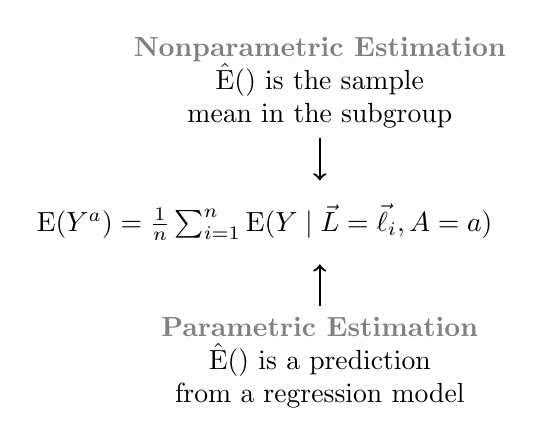
\begin{tikzpicture}[y = .7in]
\node at (0,0) {$\E(Y^a) = \frac{1}{n}\sum_{i=1}^n \E(Y\mid \vec{L} = \vec\ell_i, A = a)$};
\node[align = center] at (.7,1) {\bgray{Nonparametric Estimation}\\$\hat\E()$ is the sample\\mean in the subgroup};
\node[align = center] at (.7,-1) {\bgray{Parametric Estimation}\\$\hat\E()$ is a prediction\\from a regression model};
\draw[->, thick] (.7,.6) -- (.7, .3);
\draw[->, thick] (.7,-.6) -- (.7, -.3);
\end{tikzpicture}
\end{frame}

\begin{frame}{The parametric g-formula: Simple case}

\begin{center}
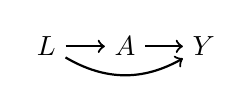
\begin{tikzpicture}
\node (l) at (0,0) {$L$};
\node (a) at (1,0) {$A$};
\node (y) at (2,0) {$Y$};
\draw[->, thick] (l) -- (a);
\draw[->, thick] (a) -- (y);
\draw[->, thick] (l) to[bend right] (y);
\end{tikzpicture}
\end{center}
\begin{tabular}{ll}
Parametric model & $\E(Y\mid L, A) = \alpha + \gamma L + \beta A$
\end{tabular} \vskip .1in \pause
Estimator for the potential outcome under treatment ($A = 1$):
$$\hat\E(Y^1) = \frac{1}{n}\sum_{i=1}^n \bigg(\hat\alpha + \hat\gamma \ell_i + \hat\beta \times 1\bigg)$$
Estimator in words:
\begin{enumerate}
\item Estimate the regression model
\item Change all treatment values to 1
\item Predict for everyone
\item Take the sample mean
\end{enumerate}

\end{frame}

\begin{frame}{The parametric g-formula: Any estimator}
Let $\hat{f}(\vec\ell,a)$ be a prediction function
$$\hat{f}(\vec\ell,a) \approx \E(Y\mid \vec{L} = \vec\ell, A = a)$$ \pause
We can convert that to an estimator for a post-intervention mean
$$\frac{1}{n}\sum_{i=1}^n \hat{f}(\vec\ell_i,a)\approx \E(Y^a)$$ \pause
Any prediction function is allowable

\end{frame}

\begin{frame}

Hill, Jennifer L. 2011.\\``\bref{https://doi.org/10.1198/jcgs.2010.08162}{Bayesian nonparametric modeling for causal inference.}"\\Journal of Computational and Graphical Statistics 20.1:217-240. \vskip .1in
\begin{itemize}
\item Binary treatment \hfill (simulated)
\item Continuous confounder $X$ \hfill (simulated)
\end{itemize} \vskip .1in
\includegraphics[width = \textwidth]{figures/hill2011_fig1}

\end{frame}

\begin{frame}
\centering
\includegraphics[height = \textheight]{figures/dorie_p1}
\end{frame}

\begin{frame}{The parametric g-formula by matching}

\begin{center}
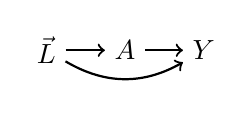
\begin{tikzpicture}
\node (l) at (0,0) {$\vec{L}$};
\node (a) at (1,0) {$A$};
\node (y) at (2,0) {$Y$};
\draw[->, thick] (l) -- (a);
\draw[->, thick] (a) -- (y);
\draw[->, thick] (l) to[bend right] (y);
\end{tikzpicture}
\end{center}
For each $i$ with $A = 1$,
\begin{itemize}
\item Find a unit $j$ with $A = 0$ that minimizes
$$d(\vec\ell_i,\vec\ell_j)$$
for some distance metric $d$
\item Impute $\E(Y\mid \vec{L} = \vec\ell_i, A = 0)$ with the observed $Y_j$
\item Estimate $\hat\delta_i = Y_i - Y_j$
\end{itemize} \vskip .1in
Estimate $\hat\E(Y^1-Y^0\mid A = 1) = \frac{1}{n_1}\sum_{i:A_i=1} \hat\delta_i$
\end{frame}

\subsection{Treatment modeling: Propensity scores}

\begin{frame}{Outcome modeling and treatment modeling}

\begin{center}
\begin{tikzpicture}[x = \textwidth]
\node[anchor = north west] at (0,0) {\begin{tikzpicture}[every node/.style={anchor = center, x = 1cm}]
\node[anchor = north west] at (-.5,1) {\bgray{Outcome modeling}};
\node (l) at (0,0) {$L$};
\node (a) at (1,0) {$A$};
\node (y) at (2,0) {$Y$};
\draw[->, line width = 1.2pt, blue] (a) -- (y);
\draw[->, line width = 1.2pt, blue] (l) to[bend right] (y);
\draw[->, thick] (l) -- (a);
\node[anchor = north west] at (-.5,-1) {1)};
\node[anchor = north west] at (-.5,-1.7) {2)};
\node[anchor = north west] at (.1,-1) {Model $\{L,A\}\rightarrow Y$};
\node[anchor = north west] at (.1,-1.7) {Impute unobserved $Y^a$};
\end{tikzpicture}}; \pause
\node[anchor = north east] at (1,0) {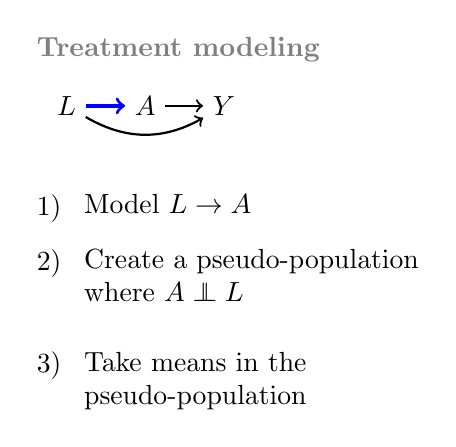
\begin{tikzpicture}[every node/.style={anchor = center, x = 1cm}]
\node[anchor = north west] at (-.5,1) {\bgray{Treatment modeling}};
\node (l) at (0,0) {$L$};
\node (a) at (1,0) {$A$};
\node (y) at (2,0) {$Y$};
\draw[->, thick] (a) -- (y);
\draw[->, thick] (l) to[bend right] (y);
\draw[->, line width = 1.2pt, blue] (l) -- (a);
\node[anchor = north west] at (-.5,-1) {1)};
\node[anchor = north west] at (-.5,-1.7) {2)};
\node[anchor = north west] at (-.5,-3) {3)};
\node[anchor = north west] at (.1,-1) {Model $L\rightarrow A$};
\node[anchor = north west, align = left] at (.1,-1.7) {Create a pseudo-population\\where $A\indep L$};
\node[anchor = north west, align = left] at (.1,-3) {Take means in the\\pseudo-population};
\end{tikzpicture}};
\end{tikzpicture}
\end{center}

\end{frame}

\begin{frame}{Intuition: Weight to a pseudo-population} \pause

Factual population:
\begin{tikzpicture}[x = \textwidth, y = .4\textheight]
\node[anchor = north] at (.45,.9) {$L = 0$};
\node[anchor = north] at (.85,.9) {$L = 1$};
\draw[rounded corners] (.3,.4) rectangle (.6,1);
\draw[rounded corners] (.7,.4) rectangle (1,1);
\node[anchor = north west, gray, font = \Huge] (unsamp) at (0,.9) {$\bullet$};
\node[anchor = west, gray] at (unsamp.east) {Untreated};
\node[anchor = north west, blue, font = \Huge] (samp) at (unsamp.south west) {$\bullet$};
\node[anchor = west, blue] (samp.east) at (samp.east) {Treated};
% L = 0
\node[gray, anchor = west, font = \Large] at (.35,.7) {$\bullet$};
\node[gray, anchor = west, font = \Large] at (.35,.6) {$\bullet$};
\node[blue, anchor = west, font = \Large] at (.35,.5) {$\bullet$};
% L = 1
\node[gray, anchor = west, font = \Large] at (.75,.7) {$\bullet$};
\node[blue, anchor = west, font = \Large] at (.75,.6) {$\bullet$};
\node[blue, anchor = west, font = \Large] at (.75,.5) {$\bullet$};
\end{tikzpicture} \vskip .05in \pause

Pseudo-population:
\begin{tikzpicture}[x = \textwidth, y = .4\textheight]
\node[anchor = north] at (.45,.9) {$L = 0$};
\node[anchor = north] at (.85,.9) {$L = 1$};
\draw[rounded corners] (.3,.4) rectangle (.6,1);
\draw[rounded corners] (.7,.4) rectangle (1,1);
\node[anchor = north west, gray, font = \Huge] (unsamp) at (0,.9) {$\bullet$};
\node[anchor = west, gray] at (unsamp.east) {Untreated};
\node[anchor = north west, blue, font = \Huge] (samp) at (unsamp.south west) {$\bullet$};
\node[anchor = west, blue] (samp.east) at (samp.east) {Treated};
% L = 0
\node[gray, anchor = west, font = \Large] at (.35,.7) {$\bullet\bullet\bullet$};
\node[gray, anchor = west, font = \Large] at (.35,.6) {$\bullet\bullet\bullet$};
\node[blue, anchor = west, font = \Large] at (.35,.5) {$\bullet\bullet\bullet$};
\draw[white, fill = white] (.4085,.55) rectangle (.47,.75);
\node[black, anchor = west, font = \footnotesize] at (.47,.7) {$w = 1.5$};
\node[black, anchor = west, font = \footnotesize] at (.47,.6) {$w = 1.5$};
\node[black, anchor = west, font = \footnotesize] at (.47,.5) {$w = 3$};
% L = 1
\node[gray, anchor = west, font = \Large] at (.75,.7) {$\bullet\bullet\bullet$};
\node[blue, anchor = west, font = \Large] at (.75,.6) {$\bullet\bullet\bullet$};
\node[blue, anchor = west, font = \Large] at (.75,.5) {$\bullet\bullet\bullet$};
\node[black, anchor = west, font = \footnotesize] at (.87,.7) {$w = 3$};
\node[black, anchor = west, font = \footnotesize] at (.87,.6) {$w = 1.5$};
\node[black, anchor = west, font = \footnotesize] at (.87,.5) {$w = 1.5$};
\draw[white, fill = white] (.8085,.45) rectangle (.87,.65);
\end{tikzpicture} \vskip .05in \pause
Each weight is the inverse probability of the observed treatment: $$w_i = \frac{1}{\P(A = a_i\mid L = \ell_i)}$$

\end{frame}

\begin{frame}[t]{Intuition: Weight to a pseudo-population} \vskip .1in
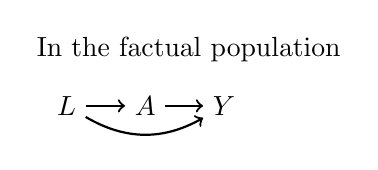
\begin{tikzpicture}
\node[anchor = north west] at (-.5,1) {In the factual population};
\node (l) at (0,0) {$L$};
\node (a) at (1,0) {$A$};
\node (y) at (2,0) {$Y$};
\draw[->, thick] (a) -- (y);
\draw[->, thick] (l) to[bend right] (y);
\draw[->, thick] (l) -- (a);
\end{tikzpicture}
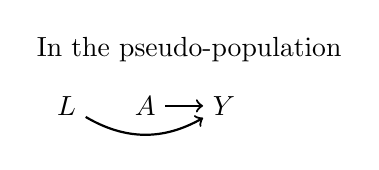
\begin{tikzpicture}
\node[anchor = north west] at (-.5,1) {In the pseudo-population};
\node (l) at (0,0) {$L$};
\node (a) at (1,0) {$A$};
\node (y) at (2,0) {$Y$};
\draw[->, thick] (a) -- (y);
\draw[->, thick] (l) to[bend right] (y);
\end{tikzpicture}
\end{frame}

\subsection{Marginal structural models}

\begin{frame}[t]{Marginal structural models} \vskip .1in
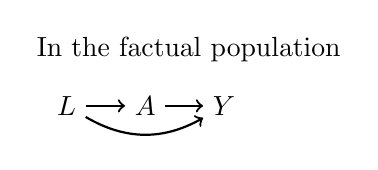
\begin{tikzpicture}
\node[anchor = north west] at (-.5,1) {In the factual population};
\node (l) at (0,0) {$L$};
\node (a) at (1,0) {$A$};
\node (y) at (2,0) {$Y$};
\draw[->, thick] (a) -- (y);
\draw[->, thick] (l) to[bend right] (y);
\draw[->, thick] (l) -- (a);
\end{tikzpicture}
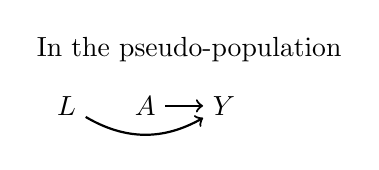
\begin{tikzpicture}
\node[anchor = north west] at (-.5,1) {In the pseudo-population};
\node (l) at (0,0) {$L$};
\node (a) at (1,0) {$A$};
\node (y) at (2,0) {$Y$};
\draw[->, thick] (a) -- (y);
\draw[->, thick] (l) to[bend right] (y);
\end{tikzpicture} \pause \vskip .2in
In the pseudo-population, estimate
$$\E(Y^a) = g(a)$$
for some parametric function $g()$ \vskip .2in \pause
Example:
$$\E(Y^a) = \alpha + \beta a$$
\end{frame}

\begin{frame}{Marginal structural models}

Useful when
\begin{itemize}
\item Treatment $A$ contains values that are sparsely populated
\begin{itemize}
\item Need to pool information from other treatment values
\end{itemize}
\item You have theory about the shape of the causal response surface $\E(Y^a)$
\item You are able to model the treatment assignment rule $\vec{L} \rightarrow A$ to create the weights
\end{itemize} \vskip .2in
Less useful when
\begin{itemize}
\item Outcome under $A = a$ is not informative about outcome under $A = a'$
\item It is hard to model $\P(A = a\mid \vec{L})$
\begin{itemize}
\item Example: Continuous rather than categorical $A$
\end{itemize}
\end{itemize}

\end{frame}

\section{Treatments that unfold over time}

\tcframe

\subsection{Treatments in many time periods}

\begin{frame}%{Treatments in many time periods}

We first addressed treatments at one time point
\begin{center}
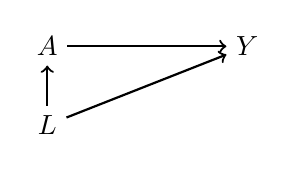
\begin{tikzpicture}[x = 1in]
\node (y) at (2,0) {$Y$};
\node (l1) at (1,-1) {$L$};
\node (a1) at (1,0) {$A$};
\draw[->, thick] (l1) -- (a1);
\draw[->, thick] (l1) -- (y);
\draw[->, thick] (a1) -- (y);
\end{tikzpicture}
\end{center}\vskip .1in \pause

Then, we addressed treatments at many time points
\begin{center}
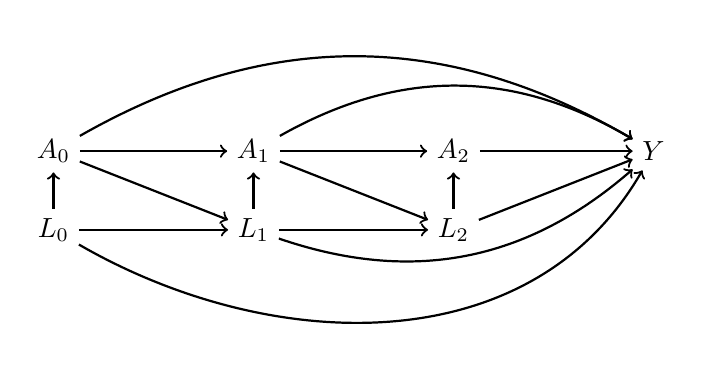
\begin{tikzpicture}[x = 1in]
\node (y) at (3,0) {$Y$};
\node (l0) at (0,-1) {$L_0$};
\node (a0) at (0,0) {$A_0$};
\draw[->, thick] (l0) -- (a0);
\draw[->, thick] (l0) to[out = 330, in = 240] (y);
\draw[->, thick] (a0) to[bend left] (y);
\node (l1) at (1,-1) {$L_1$};
\node (a1) at (1,0) {$A_1$};
\draw[->, thick] (a0) -- (a1);
\draw[->, thick] (l0) -- (l1);
\draw[->, thick] (a0) -- (l1);
\draw[->, thick] (l1) -- (a1);
\draw[->, thick] (l1) to[bend right] (y);
\draw[->, thick] (a1) to[bend left] (y);
\node (l2) at (2,-1) {$L_2$};
\node (a2) at (2,0) {$A_2$};
\draw[->, thick] (a1) -- (a2);
\draw[->, thick] (l1) -- (l2);
\draw[->, thick] (a1) -- (l2);
\draw[->, thick] (l2) -- (a2);
\draw[->, thick] (l2) -- (y);
\draw[->, thick] (a2) -- (y);
\end{tikzpicture}
\end{center}
\end{frame}

\begin{frame}{Treatments at many time points: Estimation strategy}
\begin{center}
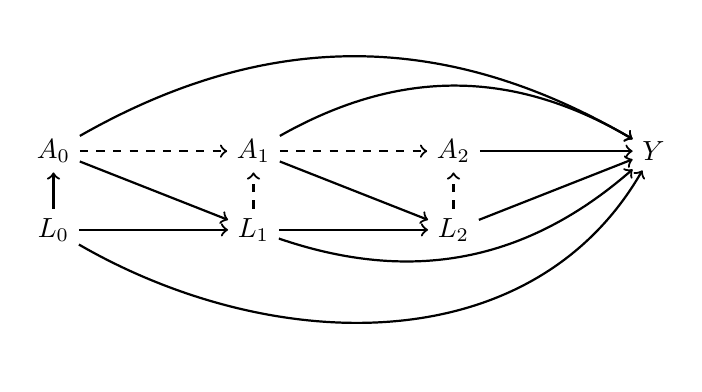
\begin{tikzpicture}[x = 1in]
\node (y) at (3,0) {$Y$};
\node (l0) at (0,-1) {$L_0$};
\node (a0) at (0,0) {$A_0$};
\draw[->, thick] (l0) -- (a0);
\draw[->, thick] (l0) to[out = 330, in = 240] (y);
\draw[->, thick] (a0) to[bend left] (y);
\node (l1) at (1,-1) {$L_1$};
\node (a1) at (1,0) {$A_1$};
\draw[->, thick, dashed] (a0) -- (a1);
\draw[->, thick] (l0) -- (l1);
\draw[->, thick] (a0) -- (l1);
\draw[->, thick, dashed] (l1) -- (a1);
\draw[->, thick] (l1) to[bend right] (y);
\draw[->, thick] (a1) to[bend left] (y);
\node (l2) at (2,-1) {$L_2$};
\node (a2) at (2,0) {$A_2$};
\draw[->, thick, dashed] (a1) -- (a2);
\draw[->, thick] (l1) -- (l2);
\draw[->, thick] (a1) -- (l2);
\draw[->, thick, dashed] (l2) -- (a2);
\draw[->, thick] (l2) -- (y);
\draw[->, thick] (a2) -- (y);
\end{tikzpicture}
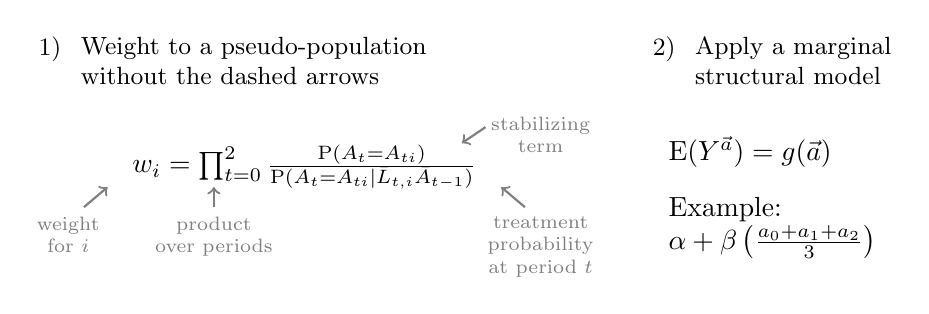
\begin{tikzpicture}[y = .2in]
\node[anchor = north west, font = \small] (one) at (-3.5, 3.5) {1)};
\node[anchor = north west, font = \small, align = left] at (one.north east) {Weight to a pseudo-population\\without the dashed arrows};
\node at (0,0) {$w_i = \prod_{t=0}^2 \frac{\P(A_t = A_{ti})}{\P(A_t = A_{ti}\mid \bar{L}_{t,i} \bar{A}_{t-1})}$};
\node[anchor = north, align = center, gray, font = \scriptsize] at (-3,-1) {weight\\for $i$};
\draw[->, thick, gray] (-2.8,-1) -- (-2.5,-.5);
\node[anchor = north, align = center, gray, font = \scriptsize] at (-1.15,-1) {product\\over periods};
\draw[->, thick, gray] (-1.15,-1) -- (-1.15,-.5);
\node[anchor = north, align = center, gray, font = \scriptsize] at (3,-1) {treatment\\probability\\at period $t$};
\draw[->, thick, gray] (2.8,-1) -- (2.5,-.5);
\node[anchor = north, align = center, gray, font = \scriptsize] at (3,1.5) {stabilizing\\term};
\draw[->, thick, gray] (2.3,1) -- (2,.6);
\node[anchor = north west, font = \small] (two) at (4.3, 3.5) {2)};
\node[anchor = north west, font = \small, align = left] at (two.north east) {Apply a marginal\\structural model};
\node[anchor = north west] at (4.5,1) {$\E(Y^{\vec{a}}) = g(\vec{a})$};
\node[anchor = north west, align = left] at (4.5,-.5) {Example:\\$\alpha + \beta\left(\frac{a_0+a_1+a_2}{3}\right)$};
\end{tikzpicture}
\end{center}

\end{frame}

\begin{frame}{Step back: When would I study treatments over time?}

\begin{itemize}
\item Treatment is assigned at many time points
\item as a function of observables up to that point
\end{itemize} \vskip .2in

Our example from class:
\begin{center}
\scalebox{.7}{
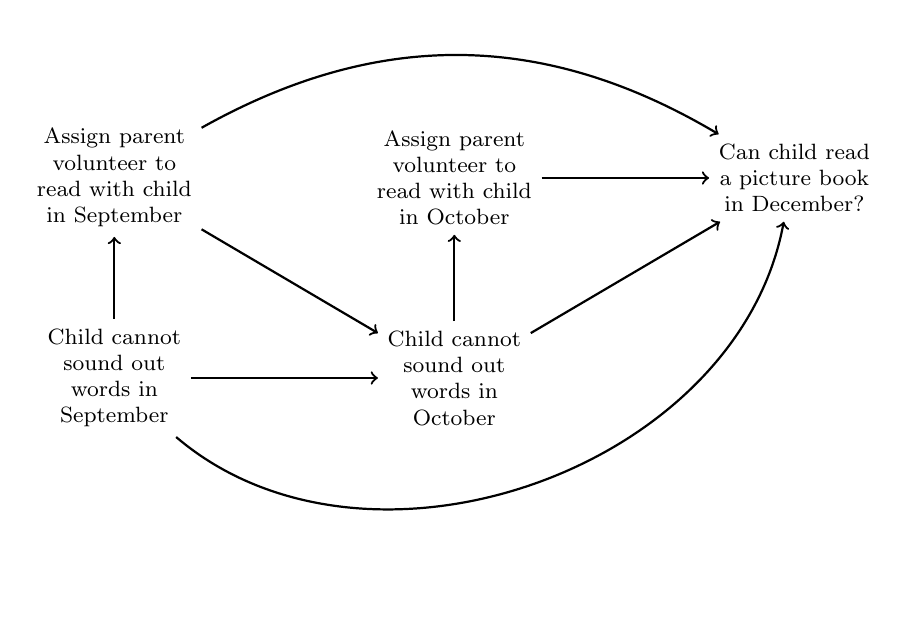
\begin{tikzpicture}[x = 1.7in, y = 1in]
\node[font = \footnotesize, align = center] (l0) at (0,-1) {Child cannot\\sound out\\words in\\September}; 
\node[font = \footnotesize, align = center] (a0) at (0,0) {Assign parent\\volunteer to\\read with child\\in September};
\draw[->, thick] (l0) -- (a0); 
\node[font = \footnotesize, align = center] (l1) at (1,-1) {Child cannot\\sound out\\words in\\October};
\draw[->, thick] (l0) -- (l1);
\draw[->, thick] (a0) -- (l1); 
\node[font = \footnotesize, align = center] (a1) at (1,0) {Assign parent\\volunteer to\\read with child\\in October};
\draw[->, thick] (l1) -- (a1); 
\node[font = \footnotesize, align = center] (y) at (2,0) {Can child read\\a picture book\\in December?};
\draw[->, thick] (l0) to[bend right = 60] (y);
\draw[->, thick] (a0) to[bend left] (y);
\draw[->, thick] (l1) -- (y);
\draw[->, thick] (a1) -- (y);
\end{tikzpicture}
}
\end{center}
\end{frame}

\subsection{Controlled direct effects}

\begin{frame}{Mediation} \pause

Methods to this point have emphasized total effects
\begin{itemize}
\item How big is the effect of $A$ on $Y$?
\item In what subgroups of $\vec{L}$ is that effect large?
\end{itemize} \vskip .2in
Mediation asks questions about how those effects come to be
\begin{itemize}
\item By what causal process does $A$ affect $Y$?
\end{itemize}

\end{frame}

\begin{frame}

\begin{center}
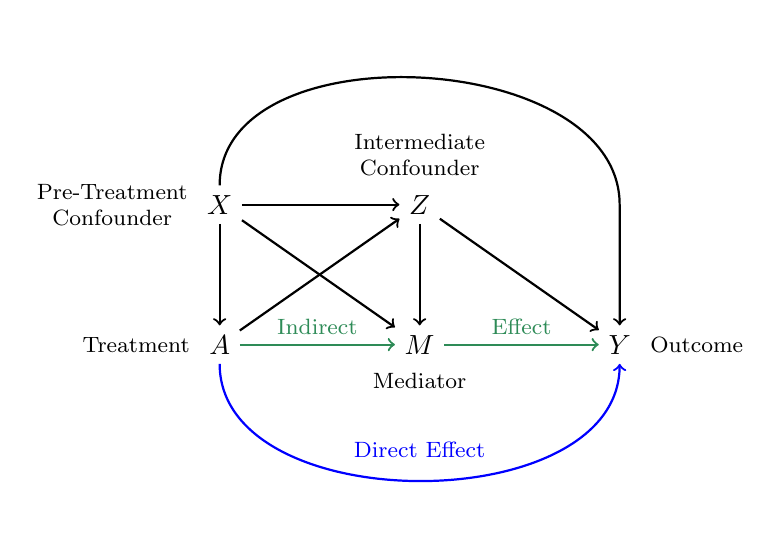
\begin{tikzpicture}[x = 1in, y = .7in]
\node (a) at (0,0) {$A$};
\node[anchor = east, font = \footnotesize] at (a.west) {Treatment};
\node (y) at (2,0) {$Y$};
\node[anchor = west, font = \footnotesize] at (y.east) {Outcome};
\node (m) at (1,0) {$M$};
\node[anchor = north, font = \footnotesize] at (m.south) {Mediator};
\draw[->, thick, blue] (a) to[bend right = 90] node[midway, above, font = \footnotesize, outer sep = 5pt] {Direct Effect} (y);
\draw[->, thick, seagreen] (a) -- node[midway, above, font = \footnotesize, seagreen] {Indirect} (m);
\draw[->, thick, seagreen] (m) -- node[midway, above, font = \footnotesize, seagreen] {Effect} (y);
\node (x) at (0,1) {$X$};
\node[anchor = east, font = \footnotesize, align = center] at (x.west) {Pre-Treatment\\Confounder};
\draw[->, thick] (x) -- (a);
\draw[->, thick] (x) -- (m);
\draw[->, thick] (x) to[out = 90, in = 90] (2,1) -- (y);
\onslide<2->{
\node (z) at (1,1) {$Z$};
\draw[->, thick] (a) -- (z);
\draw[->, thick] (x) -- (z);
\draw[->, thick] (z) -- (m);
\draw[->, thick] (z) -- (y);
\node[anchor = south, font = \footnotesize, align = center] at (z.north) {Intermediate\\Confounder};
}
\end{tikzpicture}
\end{center}

\end{frame}

\begin{frame}{Mediation: Controlled direct effects}{Test for causal paths that remain after one is blocked by an intervention.}
\bgray{Causal claim}\\
If the school librarian visits a class, that causes kids to read more.\vskip .1in \pause
\bgray{``How'' statement}\\
Happens because they become more likely to visit the school library \vskip .1in \pause
\begin{center}
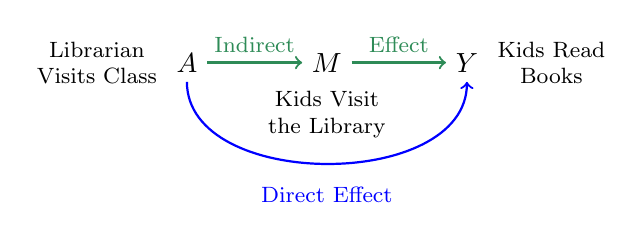
\begin{tikzpicture}[x = 1in, y = .7in, every node/.style = {anchor=center}]
\node (y) at (1.4,0) {$Y$};
\node[anchor = west, font = \footnotesize, align = center] at (y.east) {Kids Read\\Books};
\node (A) at (0,0) {$A$};
\node[anchor = east, font = \footnotesize, align = center] at (A.west) {Librarian\\Visits Class};
\node (M) at (.7,0) {$M$};
\node[anchor = north, font = \footnotesize, align = center] at (M.south) {Kids Visit\\the Library};
\draw[->, thick, seagreen] (A) -- node[midway, above, font = \footnotesize, seagreen] {Indirect} (M);
\draw[->, thick, seagreen] (M) -- node[midway, above, font = \footnotesize, seagreen] {Effect} (y);
\draw[->, thick, blue] (A) to[bend right = 90] node[midway, below, font = \footnotesize, outer sep = 5pt] {Direct Effect} (y);
\end{tikzpicture}
\end{center} \pause \vskip .1in
\bgray{Experimental test (0)} \hfill Close the library. Does $A$ affect $Y$? \\
\bgray{Experimental test (1)} \hfill Mandate library visits. Does $A$ affect $Y$? \vskip .05in
\hfill Note: Both physically manipulate $M$
\end{frame}

\subsection{Natural direct effects}

\begin{frame}{Mediation: Natural direct effects}{Decompose a total effect into direct and indirect effects} \pause

Each child has a mediator value realized under each treatment
\begin{itemize}
\item $M_i^0$: Would they visit the library if $A = 0$?
\item $M_i^1$: Would they visit the library if $A = 1$?
\end{itemize}
We cannot observe both mediator values.  \pause But what if we could? \pause

\begin{footnotesize}
$$\begin{aligned}
&\E\bigg(Y^1 - Y^0\bigg) &\text{Total effect} \\ \pause
&= \E\bigg(Y^{1M^1} - Y^{0M^0}\bigg) &\text{since }Y^{a}=Y^{aM^a} \\ \pause
&= \E\bigg(Y^{1M^1} \underbrace{- Y^{1M^0} + Y^{1M^0}}_\text{Add 0} - Y^{0M^0}\bigg) \\ \pause
&= \underbrace{\E\bigg(Y^{1M^1} - Y^{1M^0}\bigg)}_{\substack{\text{\bblue{Indirect Effect}}\\\text{(effect through $M$)}}} + \underbrace{\E\bigg(Y^{1M^0} - Y^{0M^0}\bigg)}_{\substack{\text{\bblue{Direct Effect}}\\\text{(effect not through $M$)}}}
\end{aligned}$$
\end{footnotesize}
\end{frame}

\begin{frame}{Identification: Controlled and natural direct effects}

All mediation estimands require no unmeasured confounding
\begin{center}
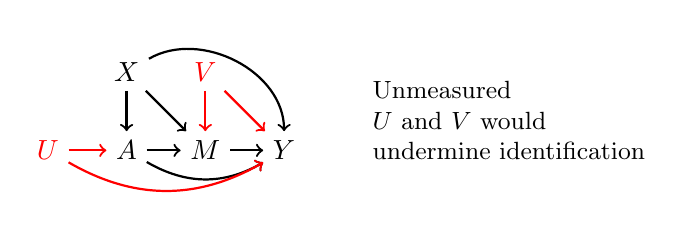
\begin{tikzpicture}
\node (a) at (0,0) {$A$};
\node (y) at (2,0) {$Y$};
\node (m) at (1,0) {$M$};
\draw[->, thick] (a) to[bend right] (y);
\draw[->, thick] (a) -- (m);
\draw[->, thick] (m) -- (y);
\node (x) at (0,1) {$X$};
\draw[->, thick] (x) -- (a);
\draw[->, thick] (x) -- (m);
\draw[->, thick] (x) to[out = 30, in = 90] (y);
\node[red] (v) at (1,1) {$V$};
\draw[->, red, thick] (v) -- (m);
\draw[->, red, thick] (v) -- (y);
\node[red] (u) at (-1,0) {$U$};
\draw[->, red, thick] (u) -- (a);
\draw[->, red, thick] (u) to[bend right] (y);
\node[anchor = north west, align = left, font = \small] at (3,1) {Unmeasured\\$U$ and $V$ would\\undermine identification};
\end{tikzpicture}
\end{center} \vskip .1in

CDE allows a measured intermediate confounder $Z$\\NDE does not allow this
\begin{center}
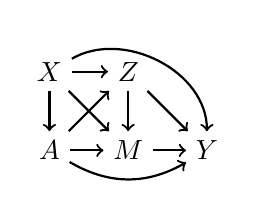
\begin{tikzpicture}
\node (a) at (0,0) {$A$};
\node (y) at (2,0) {$Y$};
\node (m) at (1,0) {$M$};
\draw[->, thick] (a) to[bend right] (y);
\draw[->, thick] (a) -- (m);
\draw[->, thick] (m) -- (y);
\node (x) at (0,1) {$X$};
\draw[->, thick] (x) -- (a);
\draw[->, thick] (x) -- (m);
\draw[->, thick] (x) to[out = 30, in = 90] (y);
\node (z) at (1,1) {$Z$};
\draw[->, thick] (a) -- (z);
\draw[->, thick] (x) -- (z);
\draw[->, thick] (z) -- (m);
\draw[->, thick] (z) -- (y);
\end{tikzpicture}
\end{center}

\end{frame}

\begin{frame}{Examples of mediation questions}
Mediation questions examine how an effect arises:\\
the causal process by which a treatment affects an outcome \vskip .05in
\begin{itemize}
\item \bref{https://doi.org/10.1177/00491241221113876}{Zhou (2022)}: The effect of enrolling in college ($A$) on earnings ($Y$) only partially operates through BA completion ($M$)
\item \bref{https://doi.org/10.1007/s13524-017-0603-1}{Wodtke \& Parbst (2017)}: The effect of neighborhood disadvantage ($A$) on children's academic achievement ($Y$) does not operate through school poverty ($M$)
\item \bref{https://sociologicalscience.com/articles-v6-11-264/}{Brand, Moore, Song, \& Xie (2019)}: The effect of parental divorce ($A$) on educational attainment ($Y$) operates partially through a drop in family income ($M$)
\end{itemize}

\end{frame}

\section{Complexities that arise in real settings}

\tcframe

\subsection{When treatment causes death: Principal stratification}

\begin{frame}{When treatment causes death: Principal stratification}

\begin{center}
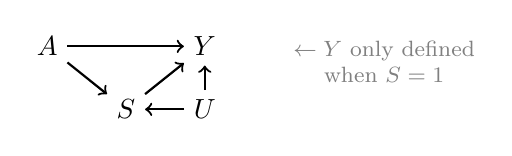
\begin{tikzpicture}
\node (a) at (0,0) {$A$};
\node (m) at (1,-.8) {$S$};
\node (y) at (2,0) {$Y$};
\node (u) at (2,-.8) {$U$};
\draw[->, thick] (a) -- (m);
\draw[->, thick] (a) -- (y);
\draw[->, thick] (m) -- (y);
\draw[->, thick] (u) -- (m);
\draw[->, thick] (u) -- (y);
\node[anchor = west, font = \footnotesize, gray, align = center] at (3,-.2) {$\leftarrow Y$ only defined\\when $S = 1$};
\end{tikzpicture}
\end{center}

\begin{itemize}
\item Suppose you have a new exercise program \hfill $A = 1$ vs $A = 0$
\item You study the effect on heart rate after 12 months \hfill $Y^1 - Y^0$
\item But only some of the people survive \hfill $S = 1$
\begin{itemize}
\item And survival was higher in your program
\end{itemize}
\end{itemize} \vskip .1in
\end{frame}

\begin{frame}{When treatment causes death: Principal stratification}
Four principal strata  \vskip .1in
\begin{enumerate}
\item Would survive regardless of treatment
\begin{itemize}
\item Our focal group: Effect of exercise on heart rate is well-defined!
\end{itemize}
\item Would not survive regardless of treatment
\item Would survive if and only if they receive the exercise program
\item Would survive if and only if the do not receive the program
\end{enumerate} \vskip .1in
\bblue{Difficulty:} We don't observe the strata.

\end{frame}

\begin{frame}{When treatment causes death: Principal stratification}

Assume \bblue{monotonicity}:\\
Exercise never hurts people. It only does nothing or helps. \vskip .2in
Survivors in the control condition would have survived regardless\vskip .05in
Survivors in the treatment condition are a mix of
\begin{itemize}
\item Survive regardless \hfill Proportion $\pi_1$
\item Survive if and only if treated \hfill Proportion $\pi_3$
\end{itemize} \vskip .2in
By estimating $A\rightarrow S$, you can estimate $\pi_1$ and $\pi_3$\\
Then, we can set-identify a range of values for
$$\E(Y^1-Y^0\mid S = \text{Survive Regardless})$$

\end{frame}

\begin{frame}{When treatment causes death: Principal stratification}

The big idea
\begin{enumerate}
\item Sometimes your sample is inherently selected\hfill (e.g., survival)
\item That needs to go on the DAG
\item If treatment causes selection, then you unavoidably condition on a post-treatment variable
\begin{itemize}
\item Which you know causes bad problems!
\end{itemize}
\item Principal stratification is the tool to set-identify an effect in a pre-treatment subgroup (e.g., survive regardless) for whom the selection variable is not post-treatment
\end{enumerate}

\begin{center}
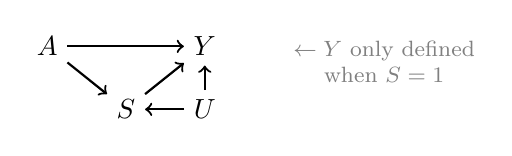
\begin{tikzpicture}
\node (a) at (0,0) {$A$};
\node (m) at (1,-.8) {$S$};
\node (y) at (2,0) {$Y$};
\node (u) at (2,-.8) {$U$};
\draw[->, thick] (a) -- (m);
\draw[->, thick] (a) -- (y);
\draw[->, thick] (m) -- (y);
\draw[->, thick] (u) -- (m);
\draw[->, thick] (u) -- (y);
\node[anchor = west, font = \footnotesize, gray, align = center] at (3,-.2) {$\leftarrow Y$ only defined\\when $S = 1$};
\end{tikzpicture}
\end{center}

\end{frame}

\subsection{When variables are measured with error}

\begin{frame}{When variables are measured with error}

When variables are measured with error,\\the DAG should include the true variable $X$\\and the measured variable $X^*$

\end{frame}

\begin{frame}{When variables are measured with error}{\bref{https://doi.org/10.1093/aje/kwp293}{Hernan \& Cole (2009)} Fig 2}

\centering
\includegraphics[height = .8\textheight]{figures/hc_fig2}

\end{frame}

\begin{frame}{When variables are measured with error}

In some cases, you can make strong assumptions\\to achieve identification despite measurement error \vskip .1in \pause

One example: \bref{https://doi.org/10.1177/0049124119875958}{Elwert \& Pfeffer~2022}

\begin{tikzpicture}[x = \textwidth]
\node[anchor = west] at (0,0) {\includegraphics[width = .4\textwidth]{figures/ep_fig1}};
\node[anchor = east] at (1,0) {$\E(Y\mid T,F) = \alpha + \beta T + \gamma F$};
\end{tikzpicture} \pause

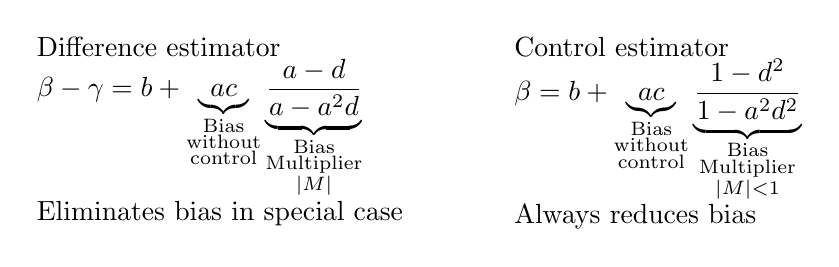
\begin{tikzpicture}[x = \textwidth]
\node[anchor = north west, align = left] at (0,0) {
Difference estimator\\
$\begin{aligned}
\beta - \gamma &= b + \underbrace{ac}_{\substack{\text{Bias}\\\text{without}\\\text{control}}}\underbrace{\frac{a - d}{a - a^2d}}_{\substack{\text{Bias}\\\text{Multiplier}\\\lvert M \rvert}}\end{aligned}$\\Eliminates bias in special case
}; \pause
\node[anchor = north west, align = left] at (.5,0) {
Control estimator\\
$\begin{aligned}
\beta &= b + \underbrace{ac}_{\substack{\text{Bias}\\\text{without}\\\text{control}}}\underbrace{\frac{1 - d^2}{1 - a^2d^2}}_{\substack{\text{Bias}\\\text{Multiplier}\\\lvert M \rvert <1}} \\
\end{aligned}$\\
Always reduces bias
};
\end{tikzpicture}
\end{frame}

\section{When exchangeability does not hold}

\tcframe

\subsection{Bounds}

\begin{frame}{When exchangeability does not hold: Bounds}

You will meet critics who do not believe exchangeability.\\
You will want to show them bounds! \vskip .1in

Setting:
\begin{itemize}
\item $A$ binary treatment
\item $Y$ bounded outcome in range $y_\text{Min} \leq Y \leq y_\text{Max}$
\end{itemize} \vskip .05in
To simplify notation,
\begin{itemize}
\item Let $\hat\bar{y}_a = \hat\E(Y\mid A = a)$ be the sample mean of $Y$ among those with $A = a$
\item Let $\hat\pi_a = \hat\P(A = a)$ be the sample proportion with $A = a$
\end{itemize}

$$\begin{aligned}
\hat\E^\text{LowerBound}(Y^a) &= \hat\pi_a\hat{\bar{y}}_a + (1 - \hat\pi_a)y_\text{Min} \\
\hat\E^\text{UpperBound}(Y^a) &= \hat\pi_a\hat{\bar{y}}_a + (1 - \hat\pi_a)y_\text{Max}
\end{aligned}$$

\end{frame}

\subsection{Difference in difference}

\begin{frame}{Difference in difference}

\begin{tikzpicture}[x = \textwidth, y = \textheight]
\node at (.5,.5) {\includegraphics[width = \textwidth]{figures/Delaware_River}};
\node[anchor = south east, font = \tiny, align = center] at (1,0) {Photo by James Loesch - https://www.flickr.com/photos/jal33/49113053632/\\CC BY 2.0, https://commons.wikimedia.org/w/index.php?curid=87207834};
\node[anchor = north west, font = \bf, white, align = left] at (.03,.64) {New Jersey\\Minimum Wage\\Rose};
\node[anchor = north east, font = \bf, white, align = right] at (1,.64) {Pennsylvania\\No change};
\end{tikzpicture}

\end{frame}

\begin{frame}[t]

\includegraphics<1>[width = \textwidth]{figures/ck_slide1.pdf}
\includegraphics<2>[width = \textwidth]{figures/ck_slide2.pdf}
\includegraphics<3>[width = \textwidth]{figures/ck_slide3.pdf}
\includegraphics<4>[width = \textwidth]{figures/ck_slide4.pdf}
\includegraphics<5>[width = \textwidth]{figures/ck_slide5.pdf}

\end{frame}

\begin{frame}[t]{Interrupted time series\footnote{Bernal, J. L., Cummins, S., \& Gasparrini, A. (2017). \bref{https://doi.org/10.1093/ije/dyw098}{Interrupted time series regression for the evaluation of public health interventions: A tutorial.} International Journal of Epidemiology, 46(1), 348-355.}} \vskip .2in
You study one unit. It is untreated. Then it is treated. \vskip .2in
\begin{center}
\includegraphics[width = .4\textwidth]{figures/parallel_trends_doubtful_4.pdf} \vskip .1in
\end{center}
\end{frame}

\begin{frame}[t]{Interrupted time series: When it becomes doubtful}
\includegraphics[width = \textwidth]{figures/its_problem_5}
\end{frame}

\subsection{Regression discontinuity}

\begin{frame}{Regression discontinuity\footnote{Cattaneo, M. D., \& Titiunik, R. (2022). \bref{https://doi.org/10.1146/annurev-economics-051520-021409}{Regression discontinuity designs.} Annual Review of Economics, 14, 821-851.}}
\begin{tikzpicture}[x = \textwidth, y = .8\textheight]
\node at (0,0) {};
\node at (1,1) {};
\node[anchor = west] (fig) at (0,.5) {\includegraphics[width = .5\textwidth]{figures/ct_fig1a}};
\node[anchor = south west, font = {\footnotesize\bf}] at (fig.north west) {Cattaneo \& Titiunik 2022 Fig 1a};
\node[anchor = north west, align = left] at (.6,.9) {\bgray{Theoretical Estimand}\\$\E(Y(1) - Y(0) \mid X = c)$};
\node[anchor = north west, align = left] at (.6,.7) {\bgray{Empirical Estimand}\\$\text{lim}_{x\downarrow c}\E(Y\mid X = x)$\\\phantom{empirical}$-$\\$\text{lim}_{x\uparrow c}\E(Y\mid X = x)$};
\node[anchor = north west, align = left] at (.6,.4) {\bgray{Identifying Assumptions}\\$\E(Y(1) \mid X = x)$ and\\$\E(Y(0) \mid X = x)$ are\\continuous at $x = c$\\{}\\and $f_X(x) > 0$ for $x$ near $c$};
\end{tikzpicture}
\end{frame}

\subsection{Synthetic control}

\begin{frame}{Synthetic control\footnote{Abadie, A., Diamond, A., \& Hainmueller, J. (2010). \bref{http://www.jenshainmueller.de/Paper/ccs.pdf}{Synthetic control methods for comparative case studies: Estimating the effect of California’s tobacco control program.} Journal of the American Statistical Association, 105(490), 493-505.}}

\begin{tikzpicture}[x = \textwidth, y = .6\textheight]
\node at (0,0) {};
\node at (1,1) {};
\node[anchor = west] at (0,.5) {\includegraphics[height = .6\textheight]{figures/synth_fig1}};
\node[anchor = north west] at (.55,1) {Can't use RD};
\node[anchor = north west, font = \small] at (.55,.92) {--- Effect at 1988 not of interest};
\node[anchor = north west] at (.55,.8) {Can't use ITS};
\node[anchor = north west, font = \small] at (.55,.72) {--- Hard to extrapolate $Y^0$ trend};
\node[anchor = north west] at (.55,.6) {Can't use DID};
\node[anchor = north west, font = \small] at (.55,.52) {--- No other state like CA};
\node[anchor = north west, align = left] (idea) at (.65,.35) {Idea: Create a\\\bblue{synthetic CA}\\to estimate\\$Y^0_\text{CA,t}$ for $t \geq 1988$};
\draw[gray, thick] (idea.north east) -- (idea.north west) -- (idea.south west) -- (idea.south east);
\end{tikzpicture}

\end{frame}

\begin{frame}{Synthetic control\footnote{Abadie, A., Diamond, A., \& Hainmueller, J. (2010). \bref{http://www.jenshainmueller.de/Paper/ccs.pdf}{Synthetic control methods for comparative case studies: Estimating the effect of California’s tobacco control program.} Journal of the American Statistical Association, 105(490), 493-505.}}

\centering
\includegraphics[height = .6\textheight]{figures/synth_fig2}

\end{frame}


\subsection{Instrumental variables}

\begin{frame}[t]{Instrumental variables: Experiment with noncompliance} \vskip .25in
\begin{center}
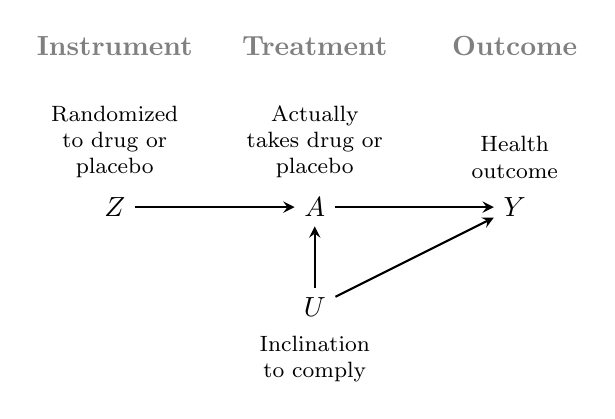
\begin{tikzpicture}[x = 1in, y = .5in]
    \node (z) at (-1,0) {$Z$};
    \node (a) at (0,0) {$A$};
    \node (y) at  (1,0) {$Y$};
    \node (u) at  (0,-1) {$U$};
    \draw[->, >=stealth, thick] (z) -- (a);
    \draw[->, >=stealth, thick] (a) --  (y);
    \draw[->, >=stealth, thick] (u) --  (a);
    \draw[->, >=stealth, thick] (u) --  (y);
    \node[anchor = south, align = center, font = \footnotesize] at (z.north) {Randomized\\to drug or\\placebo};
    \node[anchor = south, align = center, font = \footnotesize] at (a.north) {Actually\\takes drug or\\placebo};
    \node[anchor = south, align = center, font = \footnotesize] at (y.north) {Health\\outcome};
    \node[anchor = north, align = center, font = \footnotesize] at (u.south) {Inclination\\to comply};
    	\node[anchor = north, font = \bf, gray] at (-1,1.8) {Instrument};
    	\node[anchor = north, font = \bf, gray] at (0,1.8) {Treatment};
    	\node[anchor = north, font = \bf, gray] at (1,1.8) {Outcome};
  \end{tikzpicture}
\end{center}
\end{frame}

\begin{frame}[t]{Instrumental variables} \vskip .1in
\begin{center}
\scalebox{.4}{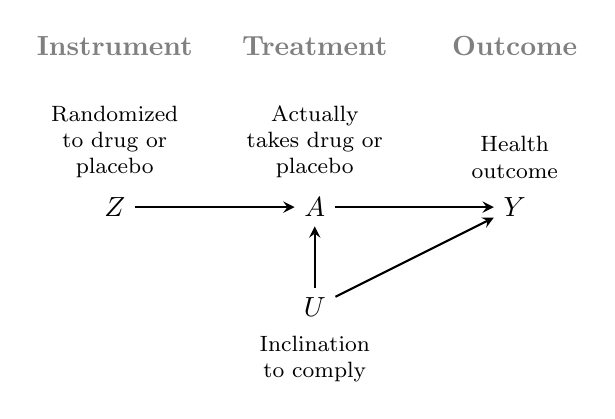
\begin{tikzpicture}[x = 1in, y = .5in]
    \node (z) at (-1,0) {$Z$};
    \node (a) at (0,0) {$A$};
    \node (y) at  (1,0) {$Y$};
    \node (u) at  (0,-1) {$U$};
    \draw[->, >=stealth, thick] (z) -- (a);
    \draw[->, >=stealth, thick] (a) --  (y);
    \draw[->, >=stealth, thick] (u) --  (a);
    \draw[->, >=stealth, thick] (u) --  (y);
    \node[anchor = south, align = center, font = \footnotesize] at (z.north) {Randomized\\to drug or\\placebo};
    \node[anchor = south, align = center, font = \footnotesize] at (a.north) {Actually\\takes drug or\\placebo};
    \node[anchor = south, align = center, font = \footnotesize] at (y.north) {Health\\outcome};
    \node[anchor = north, align = center, font = \footnotesize] at (u.south) {Inclination\\to comply};
    \node[anchor = north, font = \bf, gray] at (-1,1.8) {Instrument};
    \node[anchor = north, font = \bf, gray] at (0,1.8) {Treatment};
    \node[anchor = north, font = \bf, gray] at (1,1.8) {Outcome};
  \end{tikzpicture}}
\end{center} \vspace{-.3in}
Four principal strata
$$\begin{aligned}
\text{Compliers} \qquad& (Z\rightarrow A) = +1\quad&& (Z\rightarrow Y) = (A\rightarrow Y)\phantom{-} \\
\text{Always takers} \qquad& (Z\rightarrow A) = 0&& (Z\rightarrow Y) = 0 \\
\text{Never takers} \qquad& (Z\rightarrow A) = 0&& (Z\rightarrow Y) = 0 \\
{\text{\sout{Defiers}}} \qquad& (Z\rightarrow A) = -1&& (Z\rightarrow Y) = -(A\rightarrow Y)
\end{aligned}$$ \pause
\begin{itemize}
\item The effect $Z\rightarrow Y$ arises entirely from compliers \pause
\item The effect $Z\rightarrow A$ tells us how many compliers there are \pause
\end{itemize}
$$\E(Y^{a=1}-Y^{a=0}\mid S = \text{Complier}) = \frac{\E(Y^{z=1}-Y^{z=0})}{\E(A^{z=1}-A^{z=0})}$$

\end{frame}

\section{Recap: Causal inference in observational settings}

\tcframe

\begin{frame}
Randomized experiments are the gold standard in causal inference,\\
and for many good reasons
\end{frame}

\begin{frame}
\includegraphics[width = \textwidth]{figures/moderna_begins}\footnote{Published 27 July 2020. \url{https://www.niaid.nih.gov/news-events/phase-3-clinical-trial-investigational-vaccine-covid-19-begins}}
\end{frame}

\begin{frame}{An experimental protocol clarifies the causal estimand}
\begin{itemize}
\item Target population \hfill \textcolor{seagreen}{\checkmark}
\item Well-defined contrast between treatments \hfill \textcolor{seagreen}{\checkmark}
\item Well-defined outcome after follow-up period \hfill \textcolor{seagreen}{\checkmark}
\item Attrition is transparent \hfill \textcolor{seagreen}{\checkmark}
\item Assumptions (randomized design) support causal claims \hfill \textcolor{seagreen}{\checkmark}
\end{itemize} \vskip .4in \pause
An observational study cannot randomize.\\ \pause
Otherwise, an observational study can do all of the above.\footnote{Hern\'an, M. A., \& Robins, J. M. (2016). \bref{https://academic.oup.com/aje/article-abstract/183/8/758/1739860}{Using big data to emulate a target trial when a randomized trial is not available.} American Journal of Epidemiology, 183(8), 758-764.}
\end{frame}

\begin{frame}

A few key principles for causal inference in observational settings

\end{frame}

\begin{frame}
When you \bblue{evaluate a causal claim}, ask yourself
\begin{enumerate}
\item What is the unit of analysis?
\item What is the treatment?
\item Do the potential outcomes make sense? \hfill \textcolor{gray}{consistency}
\item Can I draw the DAG? \hfill \textcolor{gray}{exchangeability}
\item Are all treatment values plausible? \hfill \textcolor{gray}{positivity}
\end{enumerate}
\end{frame}

\begin{frame}
When you answer causal questions in \bblue{your own research}, consider
\begin{enumerate}
\item What is my causal contrast?
\begin{itemize}
\item What would it mean to assign someone to my treatment?
\end{itemize}
\item What is my target population?
\item What assumptions do I need for inference?
\begin{itemize}
\item If these assumptions, then this causal conclusion
\item The if-then statement should be airtight!
\item Then argue for those assumptions
\end{itemize}
\end{enumerate}
\end{frame}

\begin{frame}

When you \bblue{engage with new methods}, ask yourself
\begin{enumerate}
\item Counterfactuals always require assumptions.\\What assumption does this method make?
\item In what settings would this method perform well?
\item In what settings would this method perform poorly?
\item How does this method invoke key concepts I already know?
\end{enumerate}

\end{frame}

\goalsframe

\begin{frame}{What comes next?}

\begin{itemize}
\item Comments on two peers' proposals due 5pm Monday Dec 5
\item Course evaluations
\item Go out and conduct causal research!
\end{itemize}

\end{frame}

\begin{frame}{Let me know what you are thinking}

\begin{huge} \bref{https://tinyurl.com/CausalQuestions}{tinyurl.com/CausalQuestions} \end{huge}
\vskip .7in

Office hours TTh 11am-12pm and at \bref{https://calendly.com/ianlundberg/office-hours}{calendly.com/ianlundberg/office-hours}\\Come say hi!

\end{frame}


\end{document}

